% !TEX root = ../main.tex
%\begin{frame}\begin{center}
%\LARGE\textbf{Pipeline}
%\end{center}\end{frame}
\section{Pipeline}
%-------------------------------------------------------------------------------
%-------------------------------------------------------------------------------
\begin{frame}{\insertsection}
\textbf{respy}\\
\medskip
\begin{tabular}{ll}
GitHub  & \url{OpenSourceEconomics/respy}\\
Docs    & \url{respy.readthedocs.io}\\
\end{tabular}\bigskip

\textbf{estimagic}\\
\medskip
\begin{tabular}{ll}
GitHub	& \url{OpenSourceEconomics/estimagic}\\
Docs    & \url{estimagic.readthedocs.io}\\
\end{tabular}

\end{frame}
%-------------------------------------------------------------------------------
%-------------------------------------------------------------------------------
\begin{frame}{\insertsection}
	\begin{figure}
	   \lstset{basicstyle=\scriptsize\ttfamily, language=python, morekeywords={as}, ndkeywords={=}, ndkeywordstyle=\color{blue}, keywordstyle=\color{red}, commentstyle=\color{darkgrey}, emph={get_example_model, get_crit_func, get_simulate_func}, emphstyle=\color{violet}}
	   \lstinputlisting{../material/workflow.py}
	   \caption{Typical workflow}
   \end{figure}
\end{frame}
%-------------------------------------------------------------------------------
%-------------------------------------------------------------------------------
\begin{frame}{\insertsection}

	\begin{figure}[h!]\centering
	\scalebox{0.60}{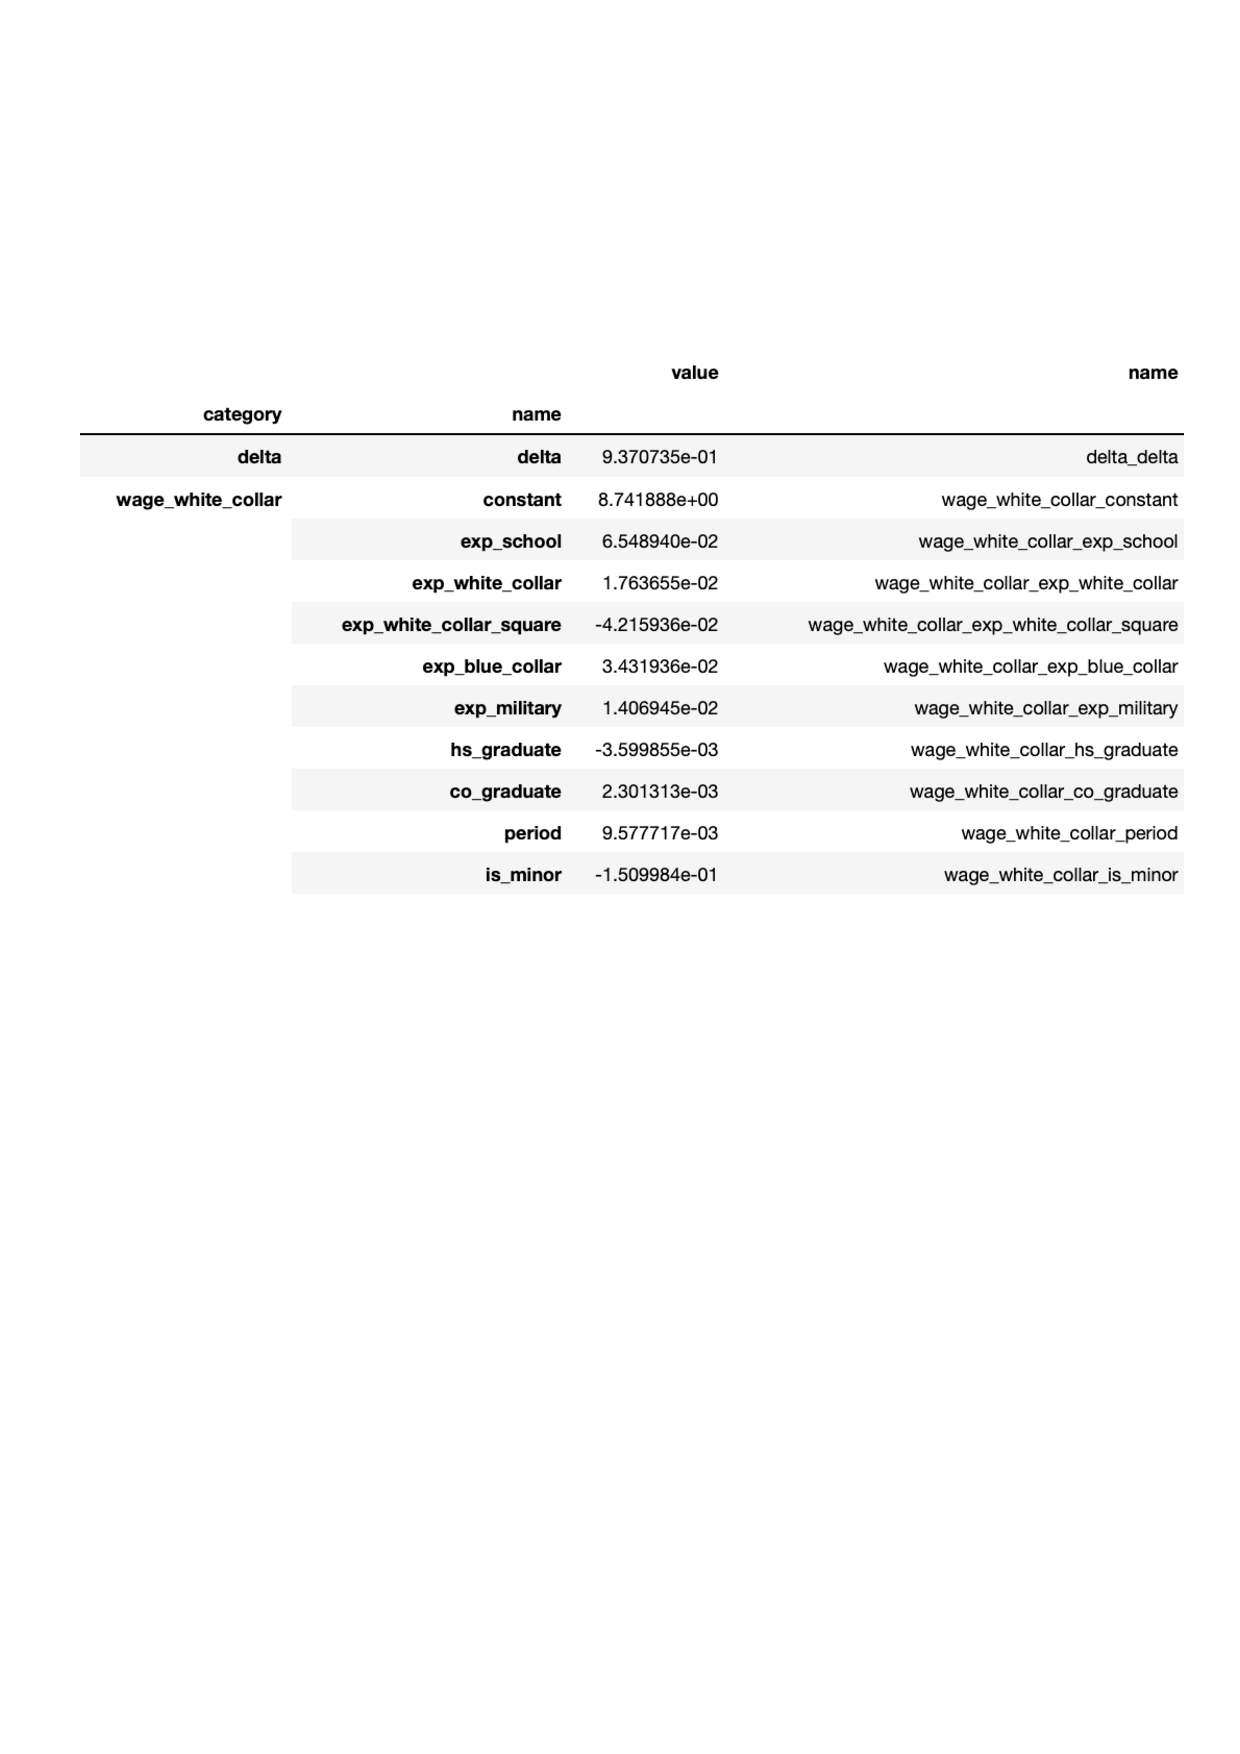
\includegraphics{crop-params}}
	\caption{Model parameterization}\label{Model parameterization}
	\end{figure}

\end{frame}
%-------------------------------------------------------------------------------
%-------------------------------------------------------------------------------
\begin{frame}{\insertsection}

	\begin{figure}[h!]\centering
	\scalebox{0.60}{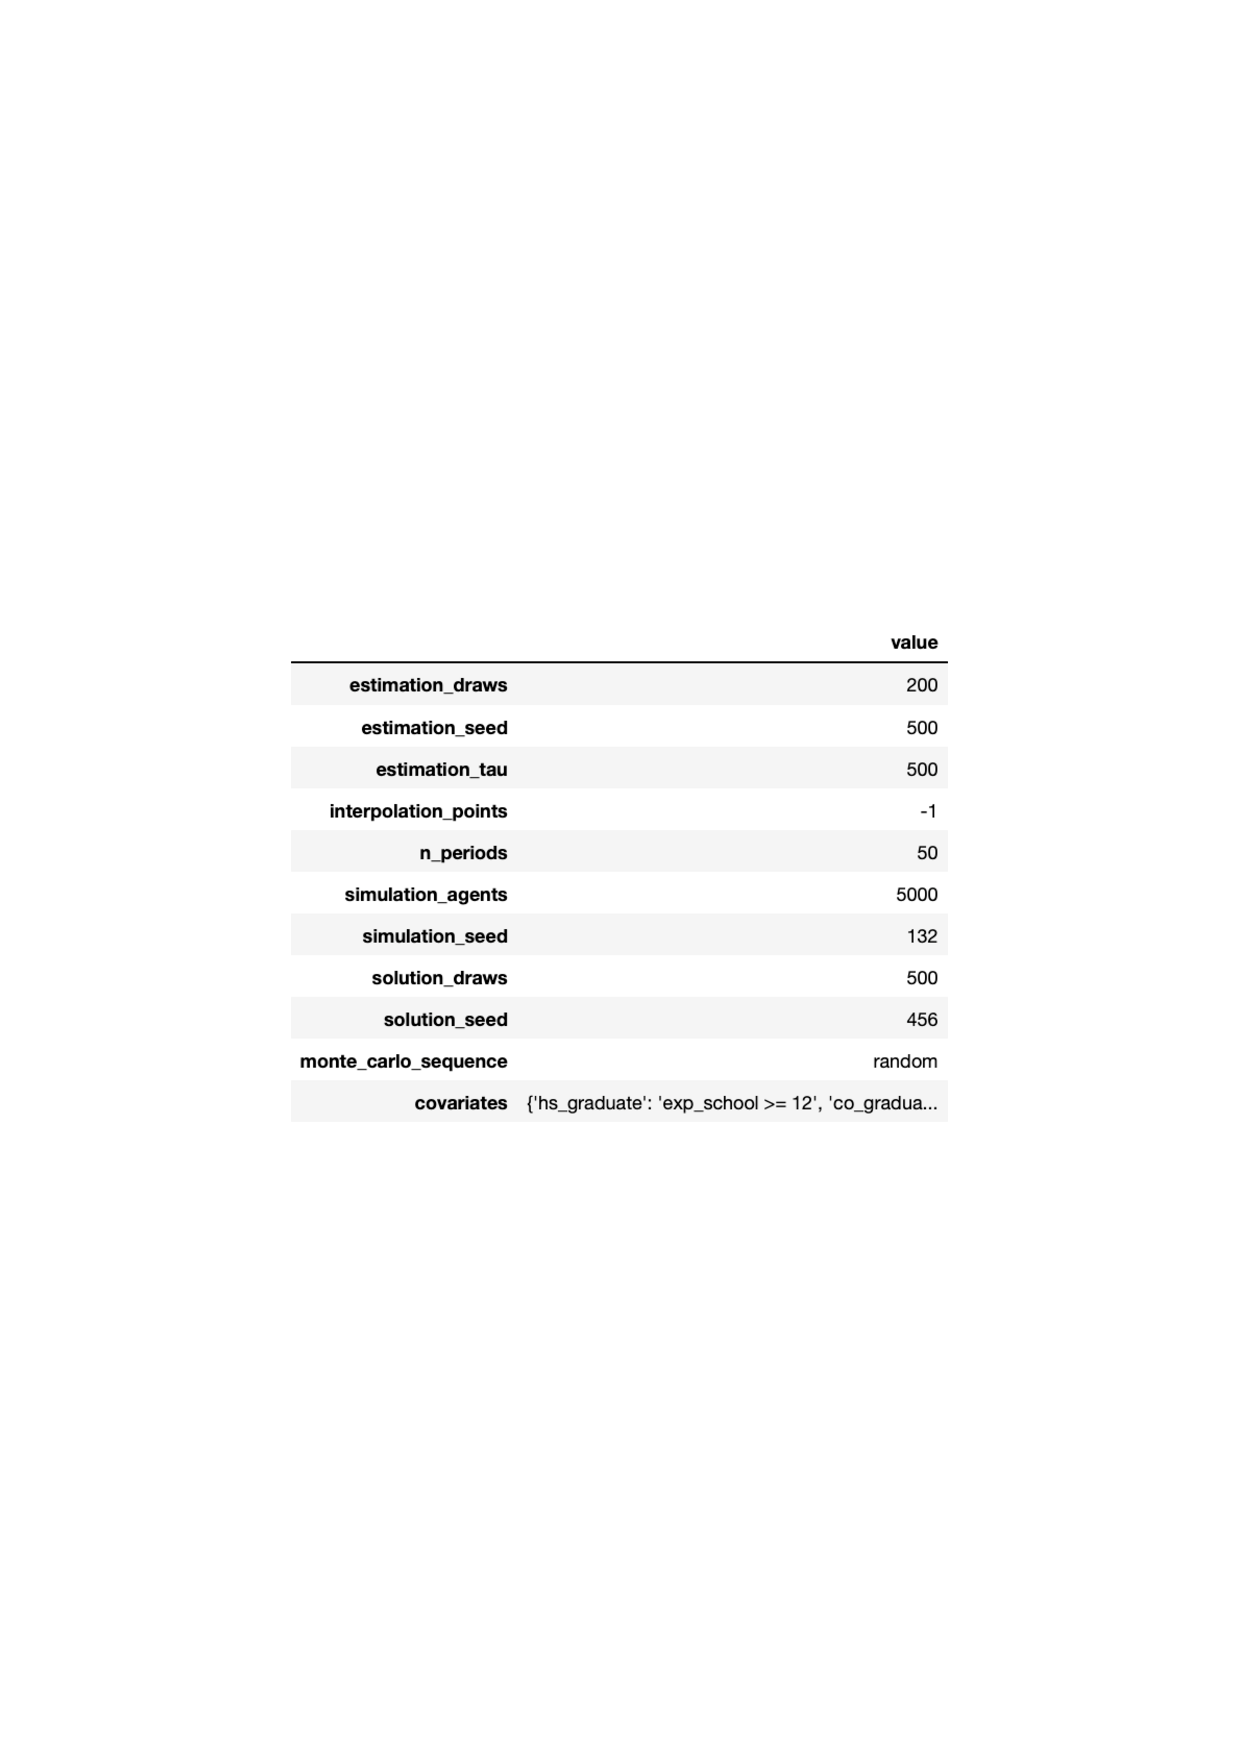
\includegraphics{crop-options}}
	\caption{Model options}\label{Model options}
\end{figure}

\end{frame}
%-------------------------------------------------------------------------------
%-------------------------------------------------------------------------------
\begin{frame}{\insertsection}

  \begin{figure}[h!]\centering
  \scalebox{0.50}{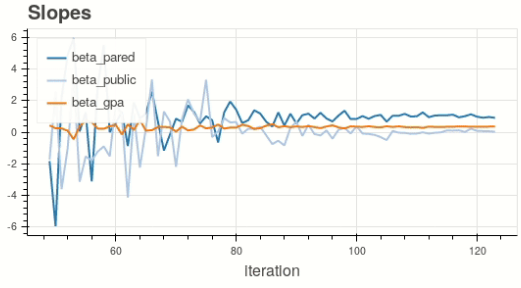
\includegraphics{crop-dashboard}}
  \caption{Dashboard}\label{Dashboard}
  \end{figure}

\end{frame}
%-------------------------------------------------------------------------------
%-------------------------------------------------------------------------------
